\documentclass{beamer}

\usepackage[utf8]{inputenc}
\usepackage{tikz}
\usetikzlibrary{calc}
\usetikzlibrary{shapes.callouts}

\usecolortheme[RGB={0,137,207}]{structure}
\setbeamertemplate{navigation symbols}{}

\title{\texttt{mathlib}: Lean's mathematical library }
\author{Johannes Hölzl \\ \includegraphics{vulogo.png}}
\date{TUM, 2018-03-21}

\newcommand{\kw}[1]{{\color{green!33!black}\ensuremath{\mathtt{#1}}}}
\newcommand{\ident}[1]{{\color{blue!33!black}\ensuremath{\mathtt{#1}}}}
\newcommand{\sect}[1]{\begin{frame}
\begin{center} \Huge{\usebeamercolor[fg]{structure} #1} \end{center}
\end{frame}
}

\begin{document}

\maketitle

\begin{frame}{Introduction}
  \begin{itemize}[<+->]
    \item (classical) mathematical library for Lean \\
      with computable exceptions, e.g.~$\mathbb{N}$, $\mathbb{Z}$, lists, \ldots
    \item Formerly distributed with Lean itself \\
          Leo wanted more flexibility
    \item Some (current) topics: \\
      Basic Datatypes, Analysis, Linear Algebra, Set Theory, \ldots
  \end{itemize}
\end{frame}

\sect{Lean}

\begin{frame}{Lean DTT (1)}
  \begin{itemize}[<+->]
    \item Basic inductives in the kernel
    \begin{itemize}
      \item Mutual and nested inductives are constructed
      \item No general fixpoint operator, no general match operator \\
        these are derived from recursors
    \end{itemize}
    \item Proof irrelevance is a definitional equality (anti-HoTT)
    \item Non-cummulative universes:
      \[ \begin{array}{ll@{\,}c@{\,}l@{\,}c@{\,}l@{\,}c@{\,}l}
        & \ident{Prop} & : & \ident{Type}_0 & : & \ident{Type}_1 & : & \cdots \\
        \pause
        \equiv & \ident{Sort}_0 & : & \ident{Sort}_1 & : & \ident{Sort}_2 & : & \cdots 
      \end{array} \]
  \end{itemize}
\end{frame}

\begin{frame}{Lean DTT (2)}
  \begin{itemize}[<+->]
    \item Subtypes (inductively defined)
      \[ \begin{array}{l}
        \ident{subtype} : \Pi (\alpha : \ident{Sort}_u),
          (\alpha \to \ident{Prop}) \to \ident{Sort}_u \\
        \{ a : \alpha \mid p\;a \} \equiv \ident{subtype}\;\alpha\;p
      \end{array} \]
    \item Quotient types (built-in)
      \[ \begin{array}{l} 
        \ident{quot} : \Pi (\alpha : \ident{Sort}_u),
          (\alpha \to \alpha \to \ident{Prop}) \to \ident{Sort}_u \\
        \alpha /_R \equiv \ident{quot}\;\alpha\;R
      \end{array} \]
    \item Mark constants \kw{noncomputable}, \\
      i.e. functions using \ident{choice}:
 \[ \kw{axiom}~\ident{choice} : \Pi (\alpha : \ident{Sort}_u), \ident{nonempty}~\alpha \to \alpha \]
  \end{itemize}
\end{frame}

\begin{frame}{Type classes in Lean}
  \begin{itemize}[<+->]
    \item Type classes are used to fill in implicit values:
    \[ \begin{array}{l}
      \ident{add} : \Pi \{\alpha : \ident{Type}\} [i : \ident{has\_add}~\alpha],~\alpha\to\alpha\to\alpha \\[1ex]
      a + b \equiv @\ident{add}~\mathbb{N}~\ident{nat.add}~a~b
    \end{array} \]
    \item Instances can depend on other instances:
      \[ \ident{ring.to\_group} : \Pi (\alpha : \ident{Type}) [i : \ident{ring}~\alpha] : \ident{group}~\alpha \]
    \item Output parameters:
    \[ \begin{array}{l@{\;:\;}l}
      \ident{has\_mem} & \ident{Type} \to \kw{out}~\ident{Type} \to \ident{Type} \\[1ex]
      \ident{set.has\_mem} & \Pi \alpha, \ident{has\_mem}~(\ident{set}~\alpha)~\alpha \\[1ex]
      \ident{fset.has\_mem} & \Pi \alpha~[i : \ident{decidable\_eq}~\alpha], \ident{has\_mem}~(\ident{fset}~\alpha)~\alpha
    \end{array} \]
    \item Default values
  \end{itemize}
\end{frame}

\sect{Library}

\begin{frame}{Library}
  \begin{itemize}
    \item Basic (computable) data
    \item Type class hierarchies:
    \begin{description}
      \item[Orders] orders, lattices
      \item[Algebraic] (commutative) groups, rings, fields
      \item[Spaces] measurable, topological, uniform, metric
    \end{description}
    \item Set theory (cardinals \& ordinals)
    \item Analysis
    \item Linear algebra
  \end{itemize}
\end{frame}

\begin{frame}{Basic (computable) data}
  \begin{itemize}[<+->]
    \item Numbers: $\mathbb{N}$, $\mathbb{Z}$ (as datatype, not quotient), $\mathbb{Q}$, \\
        $\ident{Fin} : \mathbb{N} \to \ident{Type}$
    \item $\ident{set}~\alpha := \alpha \to \ident{Prop}$
    \item $\ident{list}~\alpha$
    \item $\ident{multiset}~\alpha := \ident{list}~\alpha /_{\ident{perm}}$
    \item $\ident{finset}~\alpha := \{ m : \ident{multiset}~\alpha \mid \ident{nodup}~m \}$
    \item Big operators for $\ident{list}$, $\ident{multiset}$ and $\ident{finset}$
  \end{itemize}
\end{frame}

\begin{frame}{Set theory: Cardinals and Ordinals (Mario Carneiro)}
  \begin{itemize}[<+->]
    \item Zorn's lemma, Schröder-Bernstein, \ldots

    \item Isomorphism: \vspace{-1em} \[ \begin{array}{l} %
      \kw{structure}~\alpha \simeq \beta := \\
      (f : \alpha \to \beta) (g : \beta \to \alpha) (f\!\_g : f \circ g = id) (g\_f : g \circ f = id)
    \end{array} \]

    \item Cardinals \& ordinals are well-order
          \[
            \begin{array}{lclcl}
              \ident{cardinal}_u & : & \ident{Type}_{u+1} & := &
              \ident{Type}_u /_{\simeq}              \\
              \ident{ordinal}_u  & : & \ident{Type}_{u+1} & := &
              \ident{Well\_order}_u /_{\simeq_{ord}}
            \end{array}
          \]

    \item Semiring structure of $\ident{cardinal}$ is proved using $\simeq$ constructions

    \item $\kappa + \kappa = \kappa = \kappa * \kappa$ (for $\kappa \ge \omega$)

    \item Existence of inaccessible cardinals (i.e.~in the next universe)
  \end{itemize}
\end{frame}

\begin{frame}{Analysis}
  \begin{itemize}[<+->]
    \item Derived from Isabelle's analysis (Filters to generalize limits)
    \item Topology: open; nhds filter, closed, compact, interior, closure
    \item Uniformity: complete, totally bounded \\
      (compact $\leftrightarrow$ complete and totally bounded)
    \item Metric spaces are only rudimentary
  \end{itemize}
\end{frame}

\begin{frame}{Analysis: Analytical Structures as Complete Lattices}
  Complete lattices, \ident{map} \& \ident{comap} as category theory \emph{light}
  \begin{itemize}[<+->]
    \item $\ident{set}$, $\ident{filter}$, $\ident{topology}$, $\ident{uniformity}$, 
    and $\ident{measurable}$ form a complete lattices per type
    \[ \ident{complete\_lattice}~(\ident{topology}~\alpha) \]
    \item (Co) induced structures allow for easy constructions:
    \[ \begin{array}{l}
      \ident{map} : \Pi \{ \alpha \beta \},
        (\alpha \to \beta) \to
        (\ident{topology}~\alpha \to \ident{topology}~\beta) \\
      \ident{comap} : \Pi \{ \alpha \beta \},
        (\alpha \to \beta) \to
        (\ident{topology}~\beta \to \ident{topology}~\alpha)
    \end{array} \]
    \item Easy constructions:
    \[ \begin{array}{l}
      \ident{prod}~t_1~t_2 := \ident{comap}~\pi_1~t_1 \sqcup  \ident{comap}~\pi_2~t_2 \\
      \ident{subtype}~t~s := \ident{comap}~(\ident{subtype.val}~s)~t
    \end{array} \]
    \item Straight forward derivation of morphism rules
    \[ \begin{array}{lcl}
        \ident{cont}~f~t_{\alpha}~t_{\beta} & := &
        \ident{map}~f~t_\alpha \le t_\beta \\
        & \equiv & \forall s,~\ident{open}_\beta~s \to
             \ident{open}_\alpha~(f^{-1}[s])
      \end{array} \]
  \end{itemize}
\end{frame}

\begin{frame}{Analysis: Type Class Structure}

  \[ \begin{array}{l}
    \kw{class}~\ident{metric}~(\alpha : Type) := \ldots \\
    \kw{instance}~\ident{m2t}~(\alpha : Type)~[\ident{metric}~\alpha] :
    \ident{topology}~\alpha := \\
    \{ \ident{open}~s := \forall x \in s, \exists \epsilon > 0,
    \ident{ball}~x~\epsilon \subseteq s, \ldots \}
  \end{array} \]
\pause
  \alert{Problem}:
    $\ident{m2t}~(m_1 \times m_2) \not\equiv (\ident{m2t}~m_1) \times (\ident{m2t}~m_2)$
\pause
  \[ \begin{array}{l}
    \kw{class}~\ident{metric}~(\alpha : Type) ~\kw{extends}~\ident{topology}~\alpha := \\
    \ldots \\
    (\ident{open\_iff} : \forall s, \ident{open}~s \iff \forall x \in s, \exists \epsilon > 0,
      \ident{ball}~x~\epsilon \subseteq s)
  \end{array} \]
\pause
  Default values give a value for the topology when defining metric
\end{frame}

\begin{frame}{Analysis: Constructing Reals}
  Construct $\mathbb{R}$ using completion of $\mathbb{Q}$
  \begin{itemize}
    \item For foundational reasons metric completion is not possible \\
    \pause
      (alt: $\alpha \to \alpha \to \mathbb{Q} \to \ident{Prop}$, c.f.~Krebbers \& Spitters)
    \pause
    \item Formalize uniform spaces (using the filter library!)
    \pause
    \item Use completion on the uniform space $\mathbb{Q}$
    \pause
    \item Is it worth it? \\
    \pause
          Mario went back to Cauchy sequences...
    \pause
    \item Anyway: $\mathbb{R}$ as order \& topologically complete field
  \end{itemize}
\end{frame}

\begin{frame}{Analysis: Infinite Sum}

  \[ \left(\sum_{i:\iota} f\;i\right) = \ident{lim}_{\ident{at\_top}} \left(\lambda s,~\sum_{i \in s} f\;i\right) \]

  \begin{itemize}
    \item $\ident{at\_top} : \ident{filter}\;(\ident{finset}~\iota)$ \\
      The finite sets approaching $\ident{univ} : \ident{set}~\iota$
    \item $f : \iota \to \alpha$, the only requirement: $\alpha$ is topological monoid \\
      (e.g.~$\mathbb{R}$, normed vector spaces, \ident{ennreal}, $\mathbb{Q}$, $\mathbb{N}$, $\mathbb{Z}$, ...)
    \item $f : \left(\Sigma b : \beta, \gamma\;b\right) \to \alpha$ \qquad --- $\alpha$ regular \\
      When $\forall b, \sum_c f\;(b, c)$, and $\sum_{(b, c)} f\;(b, c)$ defined then \\
      \[ \sum_{b} \sum_{c} f\;(b, c) = \sum_{(b, c)} f\;(b, c) \]
  \end{itemize}

\end{frame}

\begin{frame}{Analysis: Measure theory}

  \[ \begin{array}{l@{\;}c@{\;}l}
    \multicolumn{3}{l}{
    \kw{structure}~\ident{measure\_space}~(\alpha : \ident{Type}_u)~[\ident{measurable\_space}~\alpha] :=} \\
    (\ident{measure'} & : & \Pi (s : \ident{set}~\alpha), \ident{measurable}~s \to \ident{ennreal}) \\
    (\ident{measure\_empty} & : & \ident{measure'}~\emptyset~\_ = 0)\\
    (\ident{measure\_UN} & : & \forall F,~(\forall i, \ident{measurable}~F_i) \to \\
      & & \hphantom{\forall F,~} \ident{measure'}~(\bigcup_i F_i)~\_ = \sum_i, \ident{measure}~(F i)~\_)
  \end{array} \]

  \begin{itemize}[<+->]
    \item What to do with non-measurable sets? \\
      In Isabelle: $\ident{measure}~\mu~s = 0$ \\
      In Lean: $\ident{measure}~\mu$ is the outer measure of $\ident{measure'}$! \\
      (hopefully: $\forall s, \int_x \ident{indicator}~s~x~\mathbf{d}\mu = \ident{measure}~\mu~s$)
    \item Developed up to Caratheodory \& Lebesgue measure
    \item Next step: Lebesgue integration
  \end{itemize}
\end{frame}

\begin{frame}{Linear Algebra}
  \[ \kw{class}~\ident{module}~(\alpha : \kw{out}~\ident{Type}_u)~(\beta : \ident{Type}_v)~[\kw{out}~\ident{ring}~\alpha] := \ldots \]
  \pause
  \begin{itemize}
    \item type class mechanism looks for $\ident{module}~\_~\beta~\_$
    \pause
    \item only one canoncial \ident{module} per type
    \pause
    \item usually $\alpha$ is fixed per theory anyway
    \pause
    \item \textbf{Problem:} (multivariate) polynomials
  \end{itemize}
  \pause
  \vspace{1em}
  \textbf{Constructions:} Subspace, Linear maps, Quotient, Product

  \pause
  \begin{example}{Isomorphism laws:}
  \[
    \frac{dom(f)}{ker(f)} \simeq_{\ell} im(f) \qquad
    \frac{s}{s \cap t} \simeq_{\ell} \frac{s \oplus t}{t}
  \]
  \end{example}

\end{frame}

\sect{Discussion}

\begin{frame}{Problems with Type Classes}
  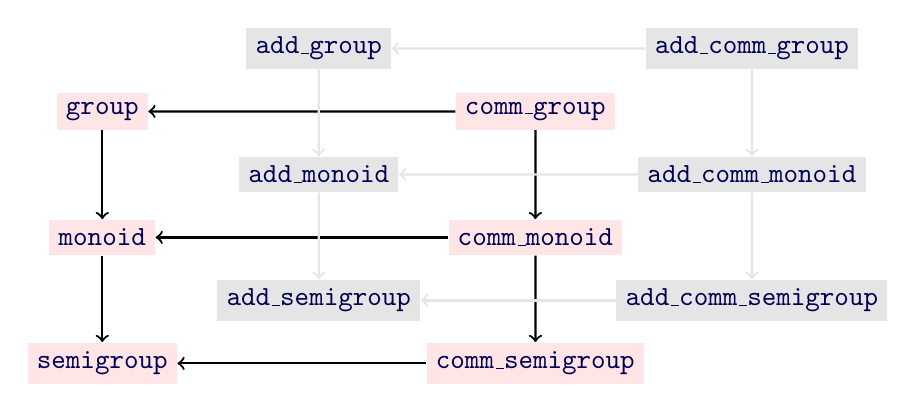
\begin{tikzpicture}[yscale=0.8, xscale=1.1, every node/.style={fill=white!90!red},
      add/.style={fill=white!90!black}]

    \onslide<1->{
      \node (s)   at (0,   -0.5) {\ident{semigroup}};
      \node (m)   at (0,   1.5) {\ident{monoid}};
      \node (g)   at (0,   3.5) {\ident{group}};

      \path[<-, thick]
      (s) edge (m)
      (m) edge (g) ;
   }

  \onslide<2->{
    \node (cs)  at (5,   -0.5) {\ident{comm\_semigroup}};
    \node (cm)  at (5,   1.5) {\ident{comm\_monoid}};
    \node (cg)  at (5,   3.5) {\ident{comm\_group}};

    \path[<-, thick]
      (s) edge (cs)
      (cs) edge (cm)
      (m) edge (cm)
      (cm) edge (cg)
      (g) edge (cg) ;

  }

  \onslide<3->{
    \node[add] (as)  at (2.5,  0.5) {\ident{add\_semigroup}};
    \node[add] (am)  at (2.5, 2.5) {\ident{add\_monoid}};
    \node[add] (ag)  at (2.5, 4.5) {\ident{add\_group}};
    \node[add] (acs) at (7.5,  0.5) {\ident{add\_comm\_semigroup}};
    \node[add] (acm) at (7.5, 2.5) {\ident{add\_comm\_monoid}};
    \node[add] (acg) at (7.5, 4.5) {\ident{add\_comm\_group}};

    \path[<-, thick, draw=white!90!black]
      (as) edge (am) edge (acs)
      (acs) edge (acm)
      (am) edge (ag) edge (acm)
      (acm) edge (acg)
      (ag) edge (acg) ;
  }

  \end{tikzpicture}
\onslide<4->{
  \begin{itemize}
    \item Currently a automated copy from \ident{group} to \ident{add\_group} \\
      instead: $[is\_group (*) (/) (\square^{-1}) 1]$ and $[is\_group (+) (-) (- \square) 0]$
    \item Mixin type classes \\
      replace \ident{comm\_monoid}, \ldots by $[is\_commutative~(*)]$
  \end{itemize}
}
\end{frame}

\begin{frame}{Problem with Universes}

  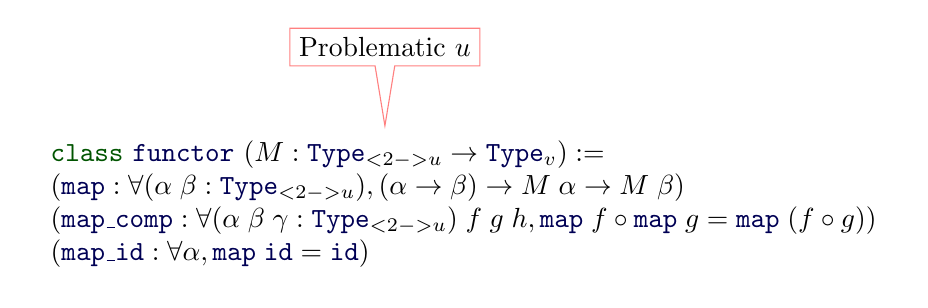
\begin{tikzpicture}
    \node (func) {
      $ \begin{array}{l}
        \kw{class}~\ident{functor}~(M : \ident{Type}_{\alert<2->{u}} \to \ident{Type}_v) := \\
        (\ident{map} : \forall (\alpha\;\beta : \ident{Type}_{\alert<2->{u}}),
          (\alpha \to \beta) \to M\;\alpha \to M\;\beta) \\
        (\ident{map\_comp} : \forall (\alpha\;\beta\;\gamma : \ident{Type}_{\alert<2->{u}})\;f\;g\;h, \ident{map}\;f \circ \ident{map}\;g =
        \ident{map}\;(f \circ g)) \\
        (\ident{map\_id} : \forall \alpha, \ident{map}\;\ident{id} = \ident{id})
      \end{array} $
    } ;
\onslide<2->{
    \node [rectangle callout,
      draw=red!50,
      callout absolute pointer={($(func) - (1,-1)$)}] at (-1, 2) {Problematic $u$} ;
      }
  \end{tikzpicture}
\onslide<3->{
If we only work with $\ident{functor}~(\ident{topology}~\alpha)$ our library is too limited,
e.g.~\ident{topology.map} allows mapping between different universes.
}
\end{frame}

\begin{frame}{Maintenance}
  \begin{itemize}
    \item Currently maintained by Mario Carneiro, me, and Jeremy Avigad \\
    \item Contributors:
    \begin{center}
      Andrew Zipperer, Floris van Doorn, Haitao Zhang, Jeremy Avigad, Johannes Hölzl, Kenny Lau,
      Kevin Buzzard, Leonardo de Moura, Mario Carneiro, Minchao Wu, Nathaniel Thomas,
      Parikshit Khanna, Robert Y. Lewis, Simon Hudon
    \end{center}
    \item Currently $\sim 54.000$ lines of Lean code
  \end{itemize}
\end{frame}

\begin{frame}{\texttt{mathlib}}

  \begin{center}
    \large A (classical) mathematical library for Lean
  \end{center}

  \begin{center}
    \url{https://github.com/leanprover/mathlib}
  \end{center}
\end{frame}

\end{document}
